% options are:
% PhD, MSc (choose one)
% beforeExam (to make the personal thanks invisible)
\documentclass[MSc,beforeExam]{iitcsthesis}

\usepackage{fontspec}
\usepackage{etoolbox}
\usepackage{polyglossia}
\usepackage{smartdiagram}
\usepackage{graphicx}
\usepackage{mathtools}
\usepackage{bidi}

\setdefaultlanguage{english}
\setotherlanguage{hebrew}
\newfontfamily\hebrewfont[Script=Hebrew]{Droid Sans Hebrew}

% For some reason, the hebrew package clashes with the amsthm package. If you need a proof environment, you can uncomment the following:
%\usepackage{amssymb} %Needed for \blacksquare. Take care not to add this package twice...
%\newenvironment{proof}[1][Proof]{\par \textbf{#1.} }{\hspace{10pt}\hfill$\blacksquare$\par}
\begin{document}

\bibliographystyle{plain}

\authorEnglish{Alex Kreimer}

\titleEnglish{Infinite Odometry}

\supervisorEnglish{The research thesis was done under the supervision
of Prof./Dr.~(First Name) (Last Name) in the Computer Science Department.}

\GregorianDateEnglish{October 2008}
\JewishDateEnglish{Tishrei 5769}

\personalThanksEnglish{Write thanks to professor and others}
\financialThanksEnglish{The generous financial support of the Technion (and someone else if you got a scholarship) is gratefully acknowledged.}

\maketitleEnglish

% The English abstract should be 200-500 words long.
\abstractEnglish In this work we revisit a problem of visual odometry
(VO). VO is the process of estimating the egomotion of the camera by
examining the changes that the motion induces on the images made by
it. The approach we propose exploits scene structure typical for that
seen by a moving car and is suitable for use in both monocular and
stereo settings. We recover rotation and translation separately, thus
dealing with two separate (smaller) problems. The rotation is
estimated by means of infinite homography which benefits from
additional data in stereo setting but may also be used in the
monocular setting. We start with an initial estimate and then refine
it using iterative procedure. After the rotation is compensated for
the translation is found by means of 1-point algorithm in stereo
setting and epipole computation for pure translational motion in
monocular setting. We evaluate our algorithm on the
KITTI~\cite{geiger2013vision} dataset.

\abbreviationsAndNotationsEnglish

\begin{tabular}{lcl}
$VO$ & --- & Visual odometry\\
$GPS$ & --- & Global Positioning System\\
$IMU$ & --- & Inertial Navigation Unit\\

\end{tabular}

%Or, if your tables are long, ``\usepackage{longtable}'' at the beginning, and then  ``\begin{longtable}[l]{lcl} ... \end{longtable}''

\section{Introduction}

\subsection{Motivation}
Visual odometry refers to the problem of recovering camera motion
based on the images taken by it. This problem naturally occurs in
robotics, wearable computing, augmented reality and automotive.

Wheel odometry, recovers the motion of the vehicle by examining and
integrating the wheel turns over time.  In similar manner, visual
odometry operates by estimating relative motion of the camera between
subsequent images by observing changes in them. Later, these estimates
are combined into a single trajectory. Just as wheel odometry, visual
odometry is subject to error accumulation over time. Contrary to wheel
odometry, visual odometry is not affected by wheel slip in rough
terrain. Visual odometry is able to produce motion estimates with
errors that are lower than those of the wheel odometry. Another
advantage of visual odometry is that cameras are low cost and low
weight sensors.  All these make visual odometry a viable supplement to
other motion recover methods such as global positioning systems (GPS)
and inertial measurement units (IMUs).

Visual odometry becomes a harder problem as the amount of detail in
the images diminishes. The images should have sufficient overlap
and the scene needs to be illuminated.  In stereo setup, the scene
must be static or the images taken at the same time. Also, video
processing incurs computational burden.

The focus of this work is on a car scenario in a stereo setup. We
evaluate our algorithm on a KITTI data-set \cite{Geiger2012}.

\begin{figure}[h]
  \centering
  \smartdiagramset{border color=none,
    uniform color list=teal!60 for 5 items,
    back arrow disabled=true,
    sequence item height=2cm,
  }
  \smartdiagram[flow diagram:horizontal]{Image sequence, Feature detection,
    Feature matching or tracking, Motion estimation, Bundle
    Adjustment}
  \caption{Common visual odometry pipeline}
\end{figure}

\subsection{Related Work}
Visual odometry are active fields of research with vast amount of
published work.  We review only the most pertinent works. Please,
refer to \cite{Scaramuzza2011} for a more complete survey.

Similar to \cite{Persson2015} visual odometry algorithms may be
clustered by four traits:
\begin{enumerate}
\item Feature-based vs direct
\item Global vs local
\item Filter based vs bundle adjustment based
\item Monocular vs stereo
\end{enumerate}

Visual odometry algorithms use large number of corner detectors
(e.g. Moravec \cite{Moravec1980}, Forstner \cite{Forstner}, Harris
\cite{Harris1987}, Shi-Tomasi \cite{Shi1994}, Fast \cite{Rosten2006})
and blob detectors (e.g., SIFT \cite{Lowe2004}, SURF
\cite{Bay2006}). Corners are faster to compute and usually are better
localized, while blobs are more robust to scale change. The choice of
a specific feature point depends mainly on the images at hand.  Motion
estimation results for different feature points are presented in
\cite{Govender2009}. In this work we choose Harris \cite{Harris1987}
corners, but this choice is not crucial. We view feature point choice
as a parameter, which needs to be determined from data (e.g., by
cross-validation).

\begin{figure}[h]
  \centering
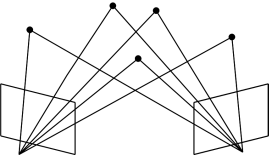
\includegraphics{5ptm2}
\caption{Matching features in two images are projections of the same
  world point}
\label{fig:5ptm}
\end{figure}

Features are either tracked \cite{Hedborg2009} or matched
\cite{Geiger2011} (i.e., freshly detected in each new frame) between
subsequent images. While early works chose to track features, most of
the current works detect and match them. The output of this stage are
pairs of image features, which are (hopefully) projections of the same
3D point in the real world, as in Figure~\ref{fig:5ptm}.

Matched features are used as an input for motion estimation procedure.
By whether the features are specified in 2-D or 3-D, the estimation
procedures, may be classified into 3-D-to-3-D (\cite{Milella2006},
3-D-to-2-D (\cite{Geiger2011}) and 2-D-to-2-D
(\cite{Nister2004}). Most of the early work was 3D-to-3D.  More recent
works \cite{Nister2004} claim that this approach is inferior to the
latter two. Popular techniques that participate in most algorithms in
some way are Essential matrix estimation and (possibly) its subsequent
decomposition \cite{Nister2004}, perspective 3-point algorithm
\cite{Kneip1991}, re-projection error minimization \cite{Geiger2011}.

Global methods \cite{Klein2007}, \cite{Newcombe2011} keep the map of
the environment and make sure that motion estimates are globally
consistent with this map, while local methods do not.  Some local
methods \cite{Badino2013} also keep track of (local) map , but the
underlying philosophy is different: global vs local.  Global methods
usually more accurate since they make use of a vast amount of
information (which, of course, comes at computational price).  Note
that accuracy does not imply robustness, since the outlier that made
it into the map may greatly skew subsequent pose estimates.

Methods that explicitly system state uncertainty tend to use filtering
mathematical machinery, e.g., \cite{Konolige2010}, \cite{Olson2003},
\cite{Kaess2008}.  Another alternative to maintain map/pose estimate
consistency is to use bundle adjustment approach \cite{Triggs2000}

Monocular systems \cite{Song} make use of a single camera, while
stereo systems \cite{Geiger2011} rely on a calibrated stereo rig. In
monocular setup the translation of the camera may only be estimated up
to scale, while in stereo all six motion parameters may be
recovered. Additional advantage of the stereo setup is more
information at each step, which may be one of the reasons why stereo
algorithms perform better.

\subsection{Our work}

Our work falls into local, feature based stereo odometry. Key ideas
that guide our work are:
\begin{itemize}
\item Prefer use of directly observed image features (as opposed to
  the computed 3-D features) as inputs for the estimation procedure.
\item Decouple rotation rotation and translation estimation into
  separate sub-problems.  Each sub-problem yields a smaller
  optimization problem which are easier to solve than a single larger
  optimization problem.
\end{itemize}

The outline of the our method:
\begin{enumerate}
\item Feature detection.  We use Harris \cite{Harris1987} features.
\item Match features to previous frame. We enforce epipolar constraint
  and use circle heuristics similar to \cite{Geiger2011}.
\item Recover camera rotation by fitting homography into the matching
  distant points.  We use 3-D at this step to decide which points are
  distant.
\item Compensate for the known rotation by application of infinite
  homography to all feature points.  This leaves us with a pure
  translation.
\item Recover the translation by minimizing the re-projection error.
\end{enumerate}

\subsection{Results Outline}
TBD

\subsection{Conclusions}
TBD
\section{Preliminaries and Notation}

\subsection{Camera model}

We consider central projection of points in space onto a plane. Let
the center of projection be the origin of the euclidean frame and let
plane $Z=f$ be the image plane. World point $\mathbf{X}=[X,Y,Z]^T$ is
projected onto the image plane by means of connecting $\mathbf{X}$ and
the center of projection and taking the intersection point of the
image plane with this line to be a projected point
$\mathbf{x}=[fX/Z,fY/Z,f]^T$


If the world point is represented by a homogeneous 4-vectors, e.g.,
$\mathbf{X} = [X,Y,Z,1]^T$, then:

\begin{equation}\label{eq:central_projection}
\begin{pmatrix}
X\\ Y\\ Z\\ 1
\end{pmatrix}
\mapsto
\begin{pmatrix}
fX\\ fY\\ Z
\end{pmatrix}
=
\begin{pmatrix}
f& & &0& \\
 &f& &0& \\
 & &1&0&
\end{pmatrix}
\begin{pmatrix}
X\\ Y\\ Z\\ 1
\end{pmatrix}
\end{equation}

Equation~\ref{eq:central_projection} assumes that the origin of coordinates in
the image plane is at principal point and that the center of
projection is at the origin of the world coordinate system.

Let the coordinates of the principal point be $c = [p_x,p_y]^T$ in the
image plane frame. Also, let the camera frame orientation be described
by $R\in SO(3)$ and its origin be the inhomogeneous vector
$C\in \mathbf{R}^3$ as seen from the world frame. Thus,
Equation~\ref{eq:central_projection} becomes:

\begin{equation}\label{eq:central_projection1}
\begin{pmatrix}
X\\ Y\\ Z\\ 1
\end{pmatrix}
\mapsto
\begin{pmatrix}
fX\\ fY\\ Z
\end{pmatrix}
=
\begin{bmatrix}
f& &p_x& \\
 &f&p_y& \\
 & &1  &
\end{bmatrix}
\begin{bmatrix}
R & -RC
\end{bmatrix}
\begin{pmatrix}
X\\ Y\\ Z\\ 1
\end{pmatrix}
\end{equation}

Denote the \emph{intrinsic parameters} matrix:
\begin{equation}
K=\begin{bmatrix}
f& &p_x& \\
 &f&p_y& \\
 & &1  &
\end{bmatrix}
\end{equation}

Denote $\mathbf{t} = -RC$ and let the \emph{extrinsic parameters}
matrix be:
\begin{equation}
\begin{bmatrix}
R & \mathbf{t}
\end{bmatrix}
\end{equation}

Putting this together and denoting \emph{camera matrix}
$P=K[R\ \mathbf{t}]$, we may write:
\begin{equation}
\mathbf{x} = K[R\ \mathbf{t}]\mathbf{X} = P\mathbf{X}
\end{equation}

Note that, $ \mathbf{X}_{cam}= [\mathsf{R}\ \mathbf{t}]\mathbf{X}$ is the
representation of $\mathbf{X}$ in the camera reference frame.

\bibliography{thesis}{}

\authorHebrew{\texthebrew{השם שלך}}

\titleHebrew{\texthebrew{כותרת התזה}}

\supervisorHebrew{\texthebrew{המחקר נעשה בהנחיית פרופ'/דר' )פרטי( )משפחה( בפקולטה למדעי המחשב.}}

\personalThanksHebrew{\texhebrew{תודות אישיות למנחים ולאחרים}}

\financialThanksHebrew{
\begin{hebrew}
אני מודה לטכניון )ולגוף שנתן מלגה אם קבלת( על התמיכה הכספית הנדיבה בהשתלמותי.
\end{hebrew}
}

\JewishDateHebrew{\texthebrew{תשרי ה'תשס"ט}}

\GregorianDateHebrew{\texthebrew{אוקטובר \beginL2008\endL}}

\maketitleHebrew

% 1000-2000 words
\abstractHebrew
\begin{hebrew}

צריך לכתוב את התקציר בעברית

\end{hebrew}
\finishedHebrew


% Actually, I found it much easier to have each chapter in a file of its own. Except for the Hebrew part, I put it all together in this example just to make things clear.

\end{document}
